\documentclass[12pt, twoside]{report}
\usepackage[utf8]{inputenc}
\usepackage{graphicx}
\usepackage{setspace}
\graphicspath{{images/}}
\usepackage[a4paper, margin=1in, bindingoffset=2cm]{geometry}
\usepackage[style=apa,sorting=nyt]{biblatex}
\DeclareLanguageMapping{american}{american-apa}
\addbibresource{ref.bib}
\usepackage{pdfpages}
\usepackage{fancyhdr}
\pagestyle{fancy}
\fancyhead{}
\fancyfoot{}
% \fancyfoot[CO, CE]{Section \thechapter}
\fancyfoot[C]{\thepage}
\renewcommand{\headrulewidth}{0pt}
% \renewcommand{\footrulewidth}{0pt}
\fancypagestyle{plain}{
    \fancyhf{} % Clear all header and footer fields
    \fancyfoot[C]{\thepage} % Center page numbers
    \renewcommand{\headrulewidth}{0pt} % Remove header line
    \renewcommand{\footrulewidth}{0pt} % Remove footer line
}

\title{
    {3D Fingerprint Reconstruction: Biometric Markers for Enhanced Fingerprint Analysis}\\
}
\date{22 August 2025}

\begin{document}
%\includepdf[pages=-]{coversheet.pdf}
\singlespacing
% Cover pages
% From the start we use Roman numerals (i, ii, etc) until we get to the first chapter.
\pagenumbering{roman}
% \pagestyle{empty}
% ---------
\begin{center}
    %\vspace*{2cm}
    \thispagestyle{empty}
    
\includegraphics[width=0.5\linewidth]{images/sheffield_newlogo.jpg}

    \vspace*{2cm}
    %\vspace*{2cm}

    \begin{Huge}
        \makeatletter
        \textbf{\@title}
        \makeatother
    \end{Huge}
 

     \vspace*{1.5cm}

  %  \begin{LARGE}
       % \makeatletter
     %   \textbf{\@author}
        %\makeatother
    %\end{LARGE}

    \vspace*{1cm}

    \begin{Large}
        Author: TeVaughn Shaw \\
        Supervised by: Dr. Hannes Saal\\
    \end{Large}

 \vspace*{2cm}

    \begin{large}
        \textit{A dissertation submitted in part requirement for the degree of} \\
        \textit{MSc Cognitive and Computational Neuroscience at the University of Sheffield}
    \end{large}

    \vspace*{1cm}
    \begin{Large}
        The University of Sheffield
    \end{Large}
    \vspace*{1cm}
    
    
    \begin{Large}
        22 August 2025
    \end{Large}
    \vspace*{1cm}
    
    %\begin{Large}
        %Word Count: 6,698
    %\end{Large}
    \vfill
\end{center}
\cleardoublepage{\thispagestyle{empty}}  % This makes sure in two-page mode the quote will be on the right
\thispagestyle{empty}

\vspace*{\fill}

\begin{singlespace}

\begin{LARGE}
    % \hspace*{3.5cm}                            % < Adjust this to align nicely with the width of your quote
    % \textbf{\textcolor{SheffieldPurple}{``}}
    
    \vspace*{-1.3\baselineskip}
    \begin{center}
        "Always ask yourself\\
        \textit{'What is the next step?'}\\
        There is always a chance to learn something\\
        new and apply it to previous knowledge."
    \end{center}
    \vspace*{-1.3\baselineskip}
    
    % \hspace*{10.5cm}                            % < Adjust this to align nicely with the width of your quote
    % \textbf{\textcolor{SheffieldPurple}{''}}
\end{LARGE}

\vspace{1cm}

\begin{large}
    \hspace*{7cm} --- Dr. Charles Hoot Jr.
\end{large}

\end{singlespace}

\vspace*{\fill}

\chapter*{Acknowledgements}
I would like to express my gratitude to my family and friends for their unwavering support throughout my academic journey. Their encouragement and understanding have been invaluable.
\chapter*{Abstract}
Reliable and accurate fingerprint recognition is important for biometric systems used in security, authentication, and personal identification. However, current technologies often rely on surface-level imaging, which can be limited by skin conditions, environmental factors, or partial contact. This study explores a new, in-vivo approach for enhancing the accuracy and robustness of fingerprint analysis by using Optical Coherence Tomography (OCT) scans of fingertip skin and reconstructed 3D meshes of the stratum corneum with associated sweat duct entry and exit points. OCT allows for high-resolution, non-invasive imaging of subsurface skin layers providing large amounts of volumetric data that can be used to capture internal features, such as sweat ducts and ridge structures. With a goal to identify consistent and trackable internal features that could serve as reliable biometric markers, we developed a pipeline for interactive region-of-interest selection using a bounding box, mesh cropping, and anatomical segmentation of internal ridge features with an interactive plane widget to ensure a clean dataset. DBSCAN was then applied to group sweat duct points, and a single centroid was calculated for each cluster to reduce the dataset while preserving key spatial information. The core of our analysis involved applying geometric metrics to these reduced centroids. We characterized the ridge geometry by examining spatial distribution, surface curvature, and normal vector orientation. Our key findings were a mean nearest-neighbor distance of $0.1259$ mm (SD = $0.0444$ mm) for the sweat duct points. We found the average mean curvature to be $5.6783$ (SD = $51.9530$), which was statistically significant ($p = 1.3726 \times 10^{-3}$). Additionally, the average normal vector dot product was $0.7891$ (SD = $0.1995$), significantly deviating from a perfectly flat surface ($p = 4.2014 \times 10^{-127}$). These results provide a quantitative description of the spatial, curvature, and orientation characteristics of internal fingerprint features to offer a strong foundation for future advancements in more reliable biometric systems.
\tableofcontents
\listoftables
\listoffigures
\chapter*{List of Abbreviations}
\begin{itemize}
    \item 2D - Two-Dimensional
    \item 3D - Three-Dimensional
    \item OCT - Optical Coherence Tomography
    \item SC - Stratum Corneum
    \item SD - Sweat Ducts
    \item VE - Viable Epidermis
    \item FAR - False Accept Rate
    \item FRR - False Reject Rate
    \item AFIS - Automated Fingerprint Identification Systems
    \item EER - Equal Error Rate
    \item CNN - Convolutional Neural Network
    \item PAD - Presentation Attack Detection
    \item TIR - Total Internal Reflection
    \item ROI - Region of Interest
    \item DBSCAN - Density-Based Spatial Clustering of Application with Noise
\end{itemize}
\clearpage
\setcounter{page}{1} 
\pagenumbering{arabic}
% \pagestyle{plain}
\doublespacing

\chapter{Introduction}
% \addcontentsline{toc}{chapter}{Introduction}

In the modern day, fingerprint recognition has become a crucial tool for biometric security, authentication, and personal identification. Biometric security systems use fingerprint recognition for its reliability and uniqueness towards fingertip ridge patterns, making them ideal for verifying identification over traditional authentication methods such as passwords and tokens, which are susceptible to loss, theft, and memory loss. The early works of \textcite{PersonalIdentificationDescription} laid the foundation of scientific study into fingerprints and their use in forensics and personal identification by introducing Level 2 features, such as minutiae points or where fingerprint ridges end or split \parencite{PersonalIdentificationDescription}. Galton discovered the existence of sweat pores on ridges; however, he did not suggest a method for their use in identification. It wasn't until 1912 that Locard introduced "poroscopy," or the comparison of sweat pores for personal identification based on their size, shape, position on the ridge, and frequency \parencite{locardLidentificationCriminelsPar1912}. In 1962, Chatterjee introduced "edgeoscopy," or the use of ridge edge shapes with other fingerprint features for individualization based on eight categories: straight, convex, peak, table, pocket, concave, angle, and others \parencite{ashbaughQuantitativequalitativeFrictionRidge1999}. The use of permanent and unique Level 3 features, such as sweat pores and ridge edge curvature, enhances minutiae-based identification.

Fingerprints have been shown to have low False Accept Rates (FAR) and False Reject Rates (FRR), making them renowned for their universality, distinction, and fast performance, leading to the creation of large-scale databases such as the FBI's over 200 million fingerprint records \parencite{chengArtificialFingerprintRecognition2006}. Automated Fingerprint Identification Systems (AFIS) have evolved into reliable systems for biometric matching, specifically in criminal investigation and various other law enforcement domains. However, conventional AFIS relies on Level 1 features, such as ridge structure and pattern, and Level 2 features. This form of 2D level surface imaging, while effective, introduces limitations that affect the robustness and security of common fingerprint recognition systems. 

One major challenge of using the outermost surface skin of the fingerprint, called the stratum corneum, is that it is susceptible to damage, skin conditions, and distortion during scanning due to the skin's elasticity or incomplete contact. Skin conditions, such as whether the skin is wet, dry, or stained during image acquisition, can lead to obscured fingerprint ridge valley patterns and overall incorrect representation of fingerprint features. Furthermore, these 2D scanners leave them highly vulnerable to presentation attacks such as spoofing, where artificial fingerprints are created using various resources such as liquid silicone rubber, gelatin, and latex. Many studies have shown that original fingerprints can be cloned and reconstructed using minutiae points by attackers and stored in user templates \parencite{sunSynchronousFingerprintAcquisition2020,liuFingerprintPresentationAttack2022,darlowEfficientInternalSurface2015}. Since the fingerprint is permanent and cannot be altered like a password, attackers collecting biometric information to breach databases is a significant issue. These limitations and underlying issues present a need for more advanced fingerprint recognition systems that look beyond surface-level imaging.

Optical Coherence Tomography (OCT) is a helpful technique that has transformed fingerprint analysis by providing a non-invasive, high-resolution 3D volumetric data of the fingertip's surface and sub-surface anatomical features. OCT systems, originally invented in medical fields such as ophthalmology and dermatology \parencite{fujimotoOpticalCoherenceTomography2000}, produce cross-sectional images called “B-scans” and depth profiles called “A-scans” to get a depiction of the multiple layers of the fingertip: the stratum corneum, viable epidermis, and papillary dermis.

Using OCT in fingerprint recognition helps address the limitations of traditional systems by extracting deeper anatomical regions in order to have more robust, secure, and accurate biometric matching. Deeper anatomical regions such as the internal fingerprint, which is formed at the viable epidermis junction, is referred to as the mother template since it is protected from outside surface injuries, deterioration from age, and environmental factors \parencite{yuMethodsApplicationsFingertip2023,dingSurfaceInternalFingerprint2021,liuLightweightNoiseRobustMethod2024}. The lack of complicated underlying biological structures in artificial fingerprints provides strong support against spoofing. OCT goes beyond traditional Level 1 and Level 2 minutiae by capturing Level 3 features such as sweat pores and ridge curvature. Sweat pores are known for their durability, consistency, and uniqueness, and align with fingerprint ridge patterns, showing potential as reliable biometric features, an idea established by Locard's poroscopy. Merging Level 3 features has shown significant improvement with performance, such as a 20 percent reduction in Equal Error Rate (EER) when combined with Level 1 and 2 features \parencite{jainPoresRidgesHighResolution2007}.
\section{Background and Related Work}
\subsection{Levels of Fingerprint}

Fingerprint analysis uses a three-level classification system with features categorized as Level 1, Level 2, and Level 3. This hierarchy is based on anatomical structure, with each level offering increasingly detailed information and serving a unique role in biometric recognition.

Level 1 fingerprint features refer to the macroscopic patterns visible on a fingerprint, such as ridge flow, whorls, loops, and arches. These features provide raw structural information for large classification instead of individual identification \parencite{maioDirectGrayscaleMinutiae1997}. For example, the Henry Classification System was developed in the late 19th century as the basis for fingerprint identification that depended on Level 1 patterns to organize a large collection of fingerprints by reducing and sorting the search space for forensic investigations (Henry, 1928).

As previously mentioned, Level 2 features add more detail by focusing on minutiae, which is where a ridge splits into two or ends abruptly. The splitting of a ridge is known as ridge bifurcations, and the abrupt ending of a ridge is known as ridge endings. They are used in modern biometric systems due to their stability and distinction for most tasks in identification \parencite{jainPoresRidgesHighResolution2007,maltoni2009handbook}. These minutiae points form the foundation for most automated fingerprint identification algorithms due to their spatial relationships and orientation to provide a framework for distinguishing individuals. The distinct appearance of these points across an individual's fingers makes them important for accurate and reliable biometric authentication.

Level 3 features offer the most detailed fingerprint information, including sweat pores, ridge contours, and underdeveloped ridges between the main ridges. Capturing these details requires high-resolution imaging, and research has shown that adding sweat pore data enhances identification accuracy, especially in forensic scenarios where only partial fingerprints are available \parencite{zhaoAdaptiveFingerprintPore2010}. Advances in fingerprint sensors and imaging technology now enable the capture of small anatomical features, boosting their use in biometric systems. This indicates that Level 3 features are crucial for high-security systems like border control checkpoints \parencite{liuOneClassFingerprintPresentation2021,sunNewApproachAutomated2023, zhangUniformRepresentationModel2024}. However, implementing Level 3-based systems remains challenging due to the high imaging resolution needed to reliably capture complex details with feature extraction algorithms \parencite{zhangSweatGlandExtraction2023,donidalabatiNovelPoreExtraction2018}.
\subsection{Prior Methods for Sweat Duct Detection}

Sweat ducts have become a popular subject of interest in advanced biometric research due to their uniqueness and stability over an individual's lifetime. Accurately detecting these ducts has been explored using a variety of methodologies involving traditional methods and deep learning techniques.

Traditional methods for detecting pores typically follow a carefully applied sequence of filtering and morphological operations on high-resolution fingerprint images to determine pore locations. \textcite{jainPoresRidgesHighResolution2007} introduced one of the earliest approaches that used Gabor filters and Mexican hat wavelet transform to enhance ridge contrast and intensify pore locations. While this method showed effectiveness for 1000 dpi resolution fingerprint images, it was tested on a small dataset, limiting its generalizability. \textcite{zhaoAdaptiveFingerprintPore2010} proposed a method to divide the fingerprint into blocks, estimate an adaptive ridge orientation in each block, and apply a match filter to accurately extract pore locations. Its adaptability boosted its accuracy over Jain; however, it struggles with dealing with distortion. \textcite{teixeiraImprovingPoreExtraction2014} introduced spatial filtering to measure distances between neighboring pores in a block and remove false positives. While it could accurately detect true pores, it struggles with determining false positives. These traditional methods, and many others, laid the foundation for sweat pore detection. Their sensitivity to noise, limited generalizability, and reliance on manual features have motivated the development of deep learning based techniques.

\textcite{donidalabatiNovelPoreExtraction2018} introduced a convolutional neural network (CNN) to detect pores using a pore intensity map with a threshold to locate pores. Their approach demonstrated that CNNs can potentially detect pores, but their capacity was limited for learning the complex patterns in fingerprint images with only two convolutional layers. \textcite{jangDeepPoreFingerprintPore2017} proposed DeepPore, a CNN with ten convolutional layers that generate pore intensity maps with spatial filtering applied to improve accuracy. The authors noted that it was trained on a small dataset, which could affect its scalability to other datasets. \textcite{anandPoreDetectionHighresolution2019} developed DeepResPore, an eighteen-layer residual learning CNN with eight residual blocks trained on over 200,000 fingerprint patch images. They tested it on two benchmark datasets and achieved state-of-the-art detection accuracy; however, its drawback was increased computational time. \textcite{sunSynchronousFingerprintAcquisition2020} created a fingerprint acquisition system combining Total Internal Reflection (TIR) and OCT to capture both surface and subsurface fingerprint structures, providing clearer visuals of sweat pores. While their work did not involve deep learning or pore detection, their technique and high-resolution data contributed to future models. The system's complexity and cost pose challenges for adoption outside research settings.

\textcite{yuNewApproachExternal2020} tackled the challenge of internal and external fingerprint registration by developing a method to minimize multisensor differences. Their approach significantly improved the alignment of external ridges with internal structures using OCT and supported accurate training models through high-quality registered data. A limitation was the difficulty in balancing resolution and acquisition speed for real-time applications. \textcite{liuRobustHighsecurityFingerprint2020} introduced a 2D recognition system that uses OCT to analyze Level 3 features primarily for anti-spoofing. They acknowledged the potential for integrating OCT-based features into learning-based classifiers. Their limitation was reliance on specialized and potentially inaccessible OCT hardware. \textcite{dingSubcutaneousSweatPore2021} presented a method using OCT to locate sweat pore positions with image analysis techniques to trace sweat duct pathways from the dermis to the fingerprint surface. Their approach offered insights into pore structure and could enhance neural network training data. However, susceptibility to image noise in deeper tissue layers affected overall accuracy. \textcite{liuNovelHighResolutionFingerprint2022} designed an approach to preserve internal and external features while maintaining detail, leading to more effective pore detection and feature extraction. Their key limitation was the trade-off between high image resolution and adequate acquisition speed in practical systems. Lastly, \textcite{sunNewApproachAutomated2023} reviewed methods and applications of fingertip biometrics using OCT. They highlighted various strategies for capturing and analyzing internal fingerprint features, emphasizing the importance of multimodal and deep learning approaches, and discussed challenges like the lack of standardized datasets and the need for efficient real-time fingerprint reconstruction systems.
\subsection{Challenges and Gaps in Current Research}
Although major advancements in fingerprint recognition systems have occurred, several important gaps remain in the research field. A key challenge hindering OCT-based fingerprint recognition is inconsistency across different devices. Recognition models often struggle to work reliably with data from new OCT machines due to small differences in imaging properties. This lack of interoperability means that these models are not easily generalizable. To make these systems practical for real-world applications, better adaptation techniques and larger datasets covering a wide range of devices are necessary. 

The inability to generalize to new threats because of poor dataset diversity represents a significant gap in Presentation Attack Detection (PAD). Many PAD methods' performance rates are limited against the constantly evolving landscape of spoofing techniques because they are frequently trained on small, homogeneous collections of spoof materials \parencite{liuFingerprintPresentationAttack2022,sunNewApproachAutomated2023,liuOneClassFingerprintPresentation2021}. It is essential to develop broader datasets that include various presentation attack instruments. This will not only improve detection accuracy for known attacks but also facilitate semi-supervised or unsupervised approaches capable of identifying spoofs they have not encountered before. Additionally, current AFIS systems lack effective integration of internal and external fingerprint features. While OCT allows imaging of internal structures such as the VE, there are no standardized protocols or efficient fusion algorithms for combining this internal data with traditional surface-level information. Merging internal and external features could significantly enhance recognition accuracy and spoof resistance; however, this area remains largely underexplored. Finally, although Level 3 features have shown promise, their practical implementation is hindered by the lack of longitudinal studies, standardized evaluation metrics, and scalable 3D processing frameworks. Future efforts in fingerprint recognition should focus on developing more advanced, adaptable, and efficient systems that surpass traditional surface imaging. This is crucial for addressing current limitations and ensuring reliable, secure, and scalable biometric authentication across diverse environments.

This paper is driven by the need to address the limitations of traditional 2D surface fingerprint systems to improve the accuracy of AFIS by using stable and secure subsurface data, such as sweat ducts and internal fingerprint ridge curvature, obtained through OCT. Using Level 3 features offers promising biometric markers that are less susceptible to distortion, damage, and spoofing. The primary objective of this work is to develop, to the best of our knowledge, the first 3D pipeline based on OCT for the extraction and analysis of 3D ridge structures and sweat ducts. Our study hypothesizes that sweat duct locations on the internal fingerprint surface are not random but follow distinctive spatial patterns, occurring at consistent distances along ridge structures, on curved ridge surfaces, and with local surface orientations that align between neighboring ducts. Our pipeline aims to address whether OCT-extracted Level 3 features provide anatomically stable and secure biometric markers for improving identification systems beyond traditional surface-level methods. 

The dissertation is structured as follows: Chapter 2 presents the proposed method; Chapter 3 presents the results; and Chapter 4 discusses the interpretation of results, limitations, and potential future directions.
\chapter{Methodology}
% \addcontentsline{toc}{chapter}{Methodology}

This section describes the framework used to investigate the anatomical organization of internal fingerprint ridges through the spatial distribution of sweat duct points acquired from 3D OCT scans. The goal of this methodology is to accurately quantify the spatial distribution of identified sweat duct points to assess the structural continuity and separability of internal ridge geometry. Having this evaluation is important for advancing the development of highly secure and spoof-resistant biometric identification systems that use Level 3 features.

\subsection{Data Acquisition}

High-resolution volumetric OCT data were obtained from fingertip scans using a Spectral Domain OCT system. The finger was positioned on a custom-made mechanical device with a flat glass slide to ensure consistent imaging during scanning. The acquisition parameters for each volumetric scan were controlled to allow detailed 3D reconstructions of the skin surface. Each scan captured a volume of 8 mm in width and 4 mm in depth. The system acquired 800 individual slices with a depth resolution of 0.005 mm. Each B-scan covered 8 mm in length and comprised 1,333 A-scans. The A-scan rate was 20,000 Hz with a sampling rate of 3E+7 Hz and 1,024 samples per A-scan with a frequency of 0.0060 mm. A plate movement of 10 mm UD was also noted.

To begin the analysis of 3D fingerprint structures from OCT data, essential Python libraries were used. Numerical and statistical operations were handled by Numpy and Scipy. For 3D processing of the data, Open3D and PyVista tools were used to complete tasks such as mesh manipulation and point cloud analysis. Sci-kit learning was applied to implement clustering algorithms to group and categorize patterns within the sweat ducts. The captured OCT volumetric data were converted into a polygon (.ply) file format in previous work. These files were loaded into the Open3D library, and high-resolution 3D Poisson surface reconstructed meshes of the SC layer were created (Kazhdan et al., 2006). The sweat duct locations, pre-processed and stored in a Python pickle file, were imported. The ducts were separated into entry points, where they emerge on the internal fingerprint surface, and exit points, where they end on the external fingerprint surface.

\subsection{Filtering and Outlier Removal}

We first focused on understanding the spatial distribution of sweat duct openings by computing the minimum distance between neighboring entry points. We achieved this by constructing a KD-tree, which reduces the computational burden of nearest neighbor searches significantly compared to brute-force methods, especially for large datasets. From these calculations, we measured the distance between each sweat duct and its closest neighbor. This measurement was important for two main reasons:

\begin{enumerate}
    \item It allowed us to identify and remove outliers from the dataset. Sweat ducts that were unusually far from their neighbors were likely to be errors or artifacts and were excluded from further analysis.
    \item It provided insights into the overall organization of the sweat duct network. By examining the distribution of distances, we could infer patterns of connectivity and continuity within the internal ridge structures.
\end{enumerate}
After the completion of these steps, we visualized the 3D fingerprint surface with respective sweat ducts using the interactive scene window in PyVista. Not only did visualizing the fingerprint mesh help as a sanity check for previous calculations, but it also aided in the next step of finding a region of interest (ROI) on the fingerprint.
\subsection{Mesh Cropping and Anatomical Segmentation}

To analyze specific features on a 3D fingerprint mesh, we start by cropping an ROI. Figure~\ref{fig:boundary_box} shows how this is done using an interactive bounding box tool, which allows a user to shape a virtual box around the desired area within the 3D mesh of the SC. The coordinates of the box are saved and used to crop down both the 3D mesh and associated sweat duct points, making this an important step because it isolates only the data relevant to the selected region of ridges and sweat ducts.
\begin{figure}[h!]
    \centering
    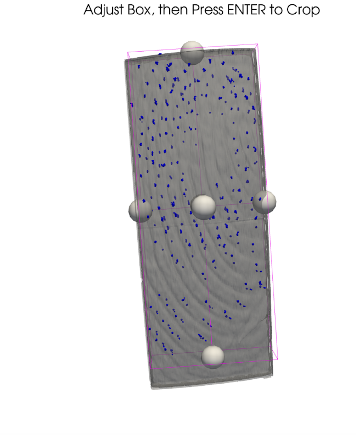
\includegraphics[width=0.5\textwidth]{images/Boundary_Box.png}
    \caption{An interactive bounding box tool used for selecting the ROI on the 3D fingerprint mesh.}
    \label{fig:boundary_box}
\end{figure}

Following the isolation of the cropped mesh and its set of sweat duct points, the next phase involved the segmentation of the dataset using an interactive plane widget. Figure~\ref{fig:cutting_plane} displays how this allows a user to define a cutting plane within the 3D visualization by positioning the plane to divide the cropped mesh and its sweat duct points along its X-axis median. The key benefit of this step is its ability to isolate a specific anatomical section of the internal fingerprint for further computational examination. Once the plane's position and orientation are confirmed, the split is computationally performed by selecting the part of the mesh and points residing beneath the plane. Additionally, any remaining pieces of the SC layer and floating points were identified and removed to give a clear visualization of the internal fingerprint surface. To clean up the high-density regions of sweat duct points, we applied the Density-Based Spatial Clustering of Application with Noise (DBSCAN) algorithm independently to the cluster of sweat duct points \parencite{esterDensityBasedAlgorithmDiscovering}. DBSCAN is a good choice for analyzing anatomical data because it can identify clusters of any shape and is resistant to noise. After clustering, we calculate a centroid for each cluster by averaging the coordinates of all the points within it. This gives us a smaller, more manageable set of representative sweat duct locations for each region.
\begin{figure}[h!]
    \centering
    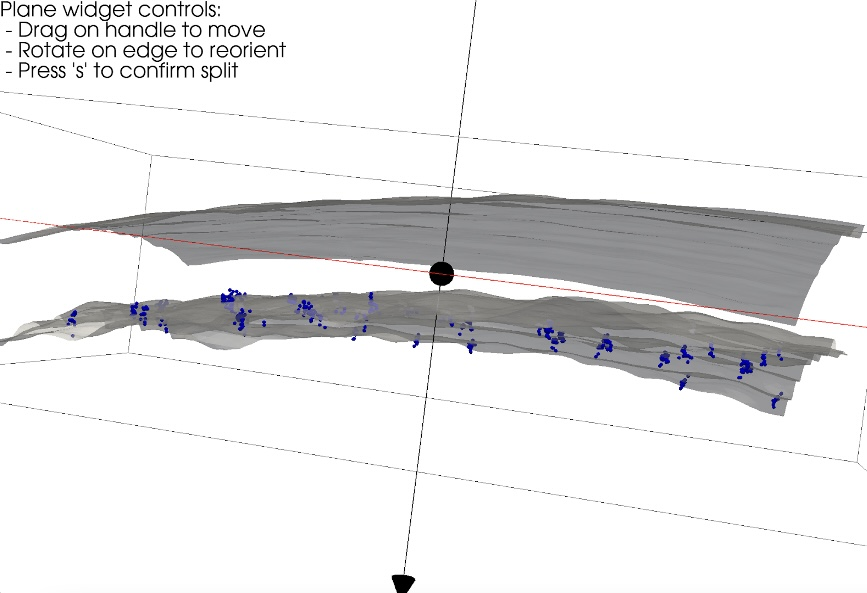
\includegraphics[width=0.8\textwidth]{images/Mesh_Splitting.jpg}
    \caption{An interactive plane widget used to segment the cropped mesh and sweat duct points along the X-axis median.}
    \label{fig:cutting_plane}
\end{figure}
\subsection{Analysis of All Sweat Duct Points}

For a detailed analysis of specific features, we conduct a comprehensive analysis of all identified sweat duct points and their local neighborhoods. The program automatically processes every reduced sweat duct point and its eight nearest neighbors to perform an aggregate, global analysis. This approach provides a broader, more accurate understanding of the internal fingerprint surface. Our analysis performed on the entire set of points consists of three parts: surface curvature, spatial distribution, and normal vector orientation. By performing this comprehensive analysis, we gain insight into the local geometry of the sweat duct points and the internal surface of the fingerprint.

We performed a curvature analysis of the mesh's local curvature to measure how much the surface bends or deviates from a flat plane. We calculated a specific mathematical measure of this bending, known as mean curvature, for each vertex on the mesh. We then extracted the curvature values for all sweat duct points and their nearest neighbors to build a color-coded visualization to display the intensity of the curvature directly on the surface of the mesh. This helps determine if the sweat ducts were located in flatter areas or regions with more curvature. We also conducted a statistical test to determine if the mean curvature of the entire set of points was significantly different from zero, which would suggest the area was not flat. We used a one-sample t-test with the null hypothesis that the region was flat, and also reported the standard deviation of the curvature values to provide a measure of the overall surface complexity.

To understand the spatial arrangement of the sweat ducts, we calculated the pairwise distances between all sweat duct points and their nearest neighbors. We visualized these distances in a heatmap to provide a clear representation of how close or far each point was from the others. Having consistent distances in the heatmap would suggest an organized, uniform pattern, whereas varying distances would indicate a more irregular distribution.

Our final analysis focused on the orientation of the sweat duct points relative to the surface. For each point on the mesh, a normal vector was calculated using surface triangulation. A normal vector is a line perpendicular to the surface at that specific point. We then calculated the dot product between the normal vector of each sweat duct point and the normal vectors of its neighbors. This value quantified the degree of alignment between the vectors. A dot product value close to 1 indicated that the vectors were nearly identically aligned, while lower values suggested a greater difference in orientation. We created a bar chart to visualize the distribution of all alignment scores. Also, we performed a one-sample t-test to determine whether the average orientation of the neighboring points was significantly different from a state of perfect alignment, such as a dot product of 1. This analysis helped us understand if the sweat ducts tended to emerge on relatively flat or uniformly sloped areas of the fingerprint.
\chapter{Results}

The analysis produced quantitative and visual outputs that describe the spatial distribution, curvature characteristics, and orientation alignment of sweat duct points across the internal fingerprint surface.
\begin{figure}[h!]
    \centering
    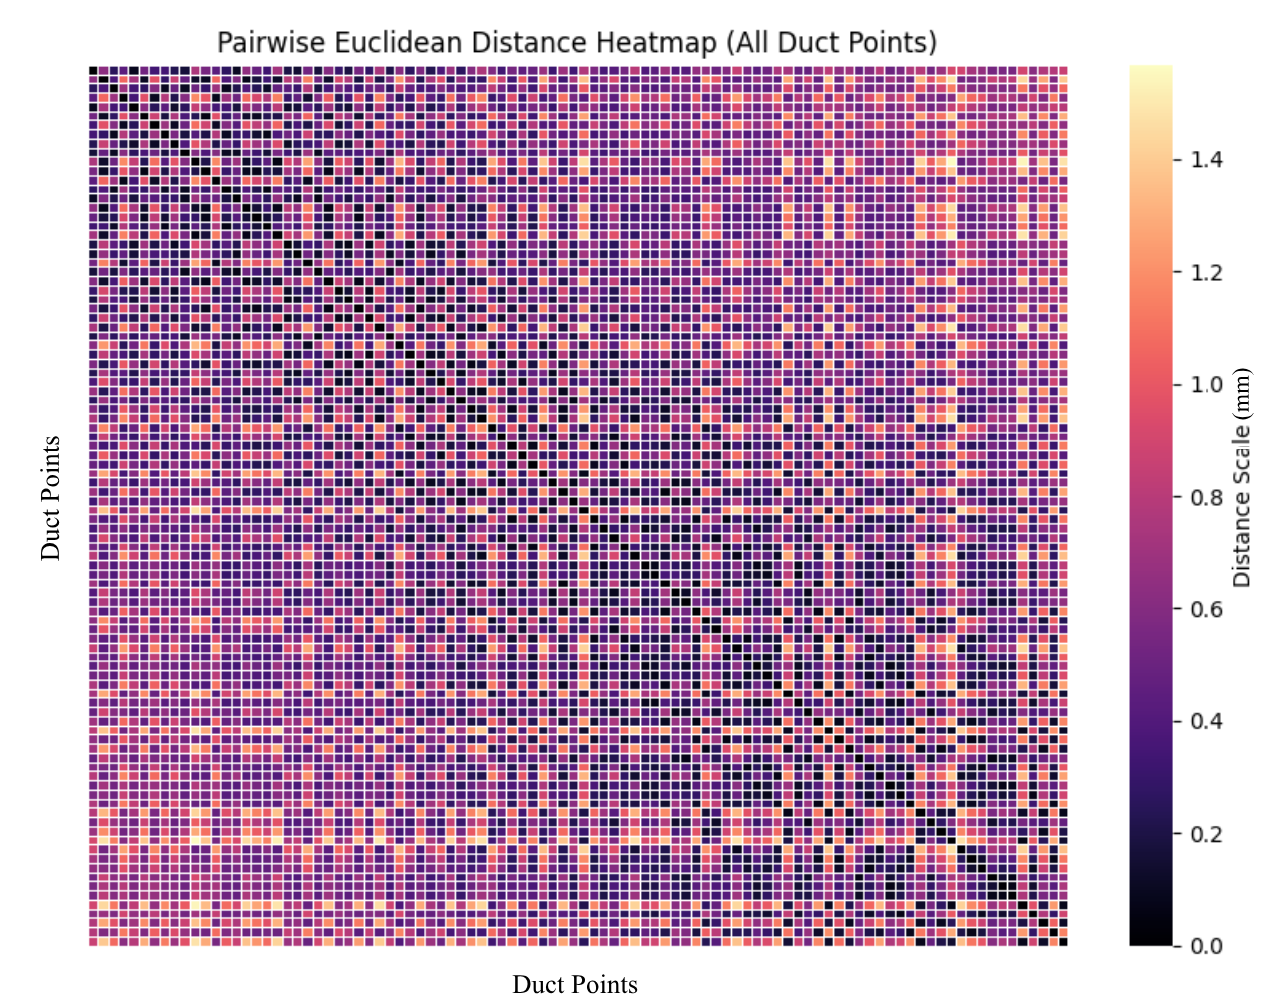
\includegraphics[width=0.9\textwidth]{images/pairwise-heatmap.png}
    \caption{Pairwise heatmap of all sweat duct points on the internal fingerprint surface.}
    \label{fig:pairwise_heatmap}
\end{figure}

Figure~\ref{fig:pairwise_heatmap} shows the pairwise Euclidean distance heatmap for all identified sweat duct points. Each axis represents a duct point index, and colors indicate the Euclidean distance between points. Distances are scaled from $0.0$ to approximately $1.5$ mm. Darker regions correspond to shorter distances, while lighter regions indicate greater separation. Repeating patterns of high- and low-distance values appear across the heatmap. The mean nearest-neighbor distance was $0.1259$ mm (SD = $0.0444$ mm).
\begin{figure}[h!]
    \centering
    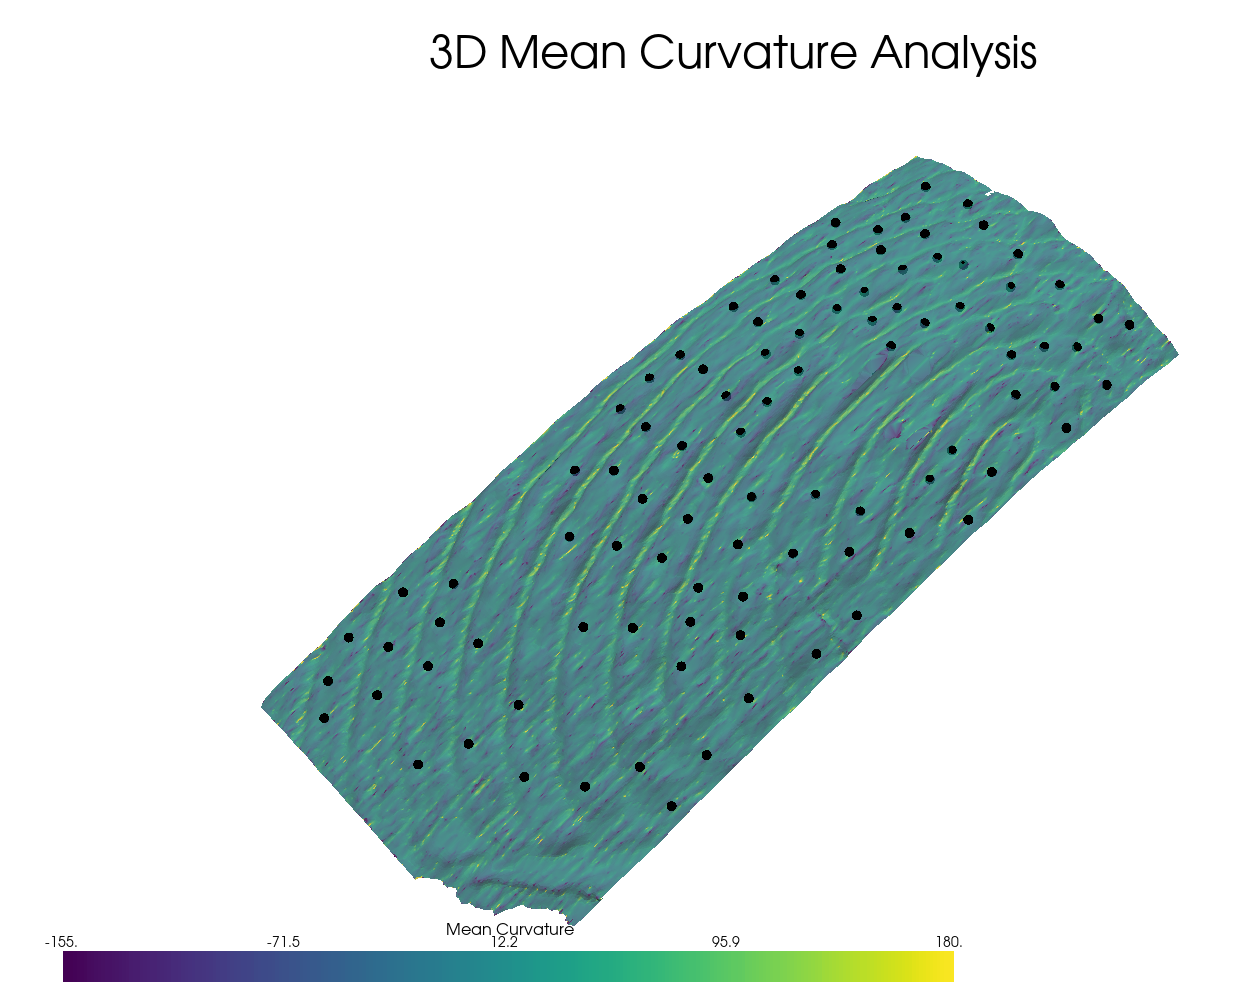
\includegraphics[width=0.9\textwidth]{images/3D_Mean_Curvature_plot.png}
    \caption{3D visualization of mean curvature values on the internal fingerprint surface.}
    \label{fig:curvature_visualization}
\end{figure}

Figure~\ref{fig:curvature_visualization} presents the results of the 3D mean curvature analysis mapped onto the internal fingerprint mesh. The curvature scale ranges from $-155.0$ mm$^{-1}$ to $180.0$ mm$^{-1}$, with cooler colors (purple to blue) representing negative curvature values, warmer colors (green to yellow) representing positive curvature values, and neutral green shades indicating near-zero curvature. Black markers indicate the positions of the sweat duct points used in the analysis. The average mean curvature measured across all sweat duct points and their nearest neighbors was $5.6783$ mm$^{-1}$ (SD = $51.9530$ mm$^{-1}$). A one-sample t-test against a null hypothesis of zero curvature produced a t-statistic of $3.2108$ and a p-value of $1.3726 \times 10^{-3}$. The null hypothesis that curvature equals zero was rejected.
\begin{figure}[h!]
    \centering
    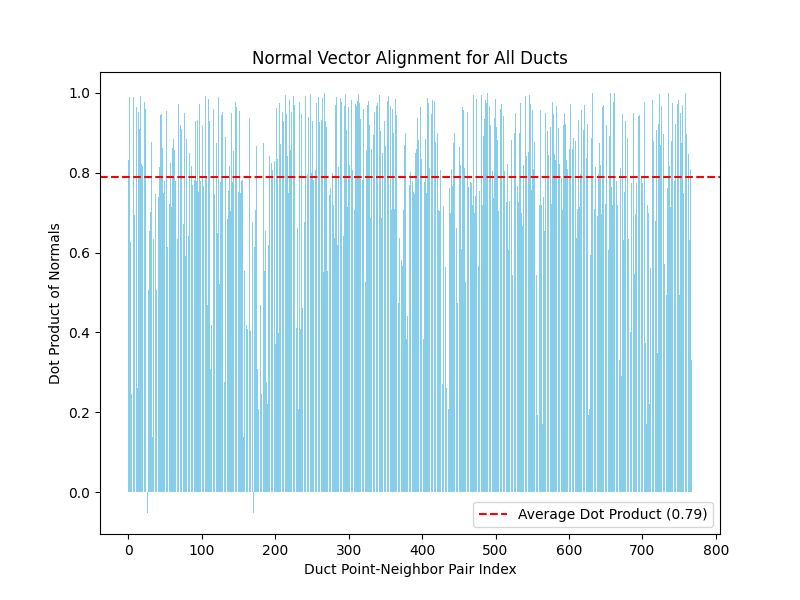
\includegraphics[width=0.9\textwidth]{images/normal_dot_product.png}
    \caption{Distribution of normal vector dot products for sweat duct points and their nearest neighbors.}
    \label{fig:normal_vector_dot_product}
\end{figure}

Figure~\ref{fig:normal_vector_dot_product} shows the distribution of dot product values between the normal vectors of sweat duct points and those of their neighbors. Each bar corresponds to a single point-neighbor pair, with the vertical axis representing the dot product value and the horizontal axis indexing all such pairs. The dashed horizontal red line marks the mean dot product value of $0.7891$. The average dot product of normal vectors was $0.7891$ (SD = $0.1995$). A one-sample t-test comparing the observed mean to a value of perfect alignment ($1.0$) produced a t-statistic of $-29.2802$ and a p-value of $4.2014 \times 10^{-127}$. The null hypothesis of perfect alignment was rejected.
\subsection{Subset Analysis}

A subset of the dataset ($N = 10$) was also analyzed. The mean nearest-neighbor distance was $0.1696$ mm (SD = $0.0679$ mm). The average mean curvature was $4.7877$ mm$^{-1}$ (SD = $31.4448$ mm$^{-1}$), with a t-statistic of $1.5073$ and a p-value of $1.3496 \times 10^{-1}$. The null hypothesis that curvature equals zero was not rejected. The average dot product of normal vectors was $0.8553$ (SD = $0.1458$), with a t-statistic of $-9.2552$ and a p-value of $1.3478 \times 10^{-14}$. The null hypothesis of perfect alignment was rejected.
\chapter{Discussion}
\subsection{Interpretation of Results}

This work aimed to investigate whether 3D OCT data could be used to extract and analyze Level 3 fingerprint features, specifically sweat ducts and internal ridge geometry, in a manner that could enhance biometric security systems. Traditional fingerprint recognition systems primarily rely on Level 1 and Level 2 features. These systems are limited by their dependence on surface imaging. The findings of this project provide initial evidence that internal anatomical features obtained from OCT scans offer distinct patterns. These patterns could serve as stable and spoof-resistant biometric markers. 

\begin{table}[ht]
\centering
\caption{Summary of quantitative results for the full dataset and subset of sweat duct points.}
\label{tab:results}
\resizebox{\textwidth}{!}{%
\begin{tabular}{lcccccc}
\hline
\textbf{Measure} & \textbf{Dataset} & \textbf{Mean} & \textbf{SD} & \textbf{t} & \textbf{p} & \textbf{Null Hypothesis} \\
\hline
Nearest-Neighbor Distance (mm) & Full & 0.1259 & 0.0444 & -- & -- & Not tested \\
                               & Subset & 0.1696 & 0.0679 & -- & -- & Not tested \\
Mean Curvature (mm$^{-1}$)     & Full & 5.6783 & 51.9530 & 3.2108 & 1.37 $\times$ 10$^{-3}$ & Rejected \\
                               & Subset & 4.7877 & 31.4448 & 1.5073 & 1.35 $\times$ 10$^{-1}$ & Not rejected \\
Normal Vector Dot Product      & Full & 0.7891 & 0.1995 & -29.2802 & 4.20 $\times$ 10$^{-127}$ & Rejected \\
                               & Subset & 0.8553 & 0.1458 & -9.2552 & 1.35 $\times$ 10$^{-14}$ & Rejected \\
\hline
\end{tabular}%
}
\end{table}

The quantitative results from the spatial distribution analysis show that sweat ducts are not randomly dispersed across the internal fingerprint surface. The mean nearest-neighbor distance across all sweat ducts was about 0.126 mm, with a relatively small standard deviation. This consistency indicates a stable spacing pattern. The finding aligns with prior anatomical studies that suggest sweat ducts follow the course of ridges and appear at relatively uniform intervals. Subset analysis, which examined ten sweat ducts, showed a slightly higher mean distance of 0.170 mm. This suggests that smaller samples reflect local variation while the overall population maintains a stable pattern. Such regularity is valuable for biometric recognition. It means sweat duct arrangements may be predictable enough to help matching algorithms, but still unique enough between individuals to serve as identifying characteristics. The curvature analysis further supports the potential of these features. Sweat duct points were found in regions of the ridge that are not perfectly flat. Statistical testing confirmed a significant deviation from zero curvature. This shows that sweat ducts tend to be located along ridge parts that have slight 3D contours. From a practical perspective, this curvature data adds spatial context for matching. It allows algorithms to encode not only the x and y positions of sweat ducts, but also their orientation on a curved surface. Having this depth of information could make it more difficult for attackers to create convincing spoofing attacks. A counterfeit fingerprint would need to replicate both curvature distribution and sweat duct spacing.

The normal vector analysis provides additional insight by examining how sweat duct orientations align. An average dot product of about 0.79 shows that most sweat ducts have similar directions compared to their neighbors. Some variation still exists across the fingerprint. The subset analysis showed a higher mean alignment of 0.86. This suggests that smaller fingerprint regions are more uniform in topography. Anatomically, this means that duct emergence angles are influenced by the microstructure of the ridge in a local area, while still exhibiting subtle changes along the ridge. These findings are significant because they reveal a multi-dimensional set of parameters: spacing, curvature, and orientation. These could be integrated into more advanced fingerprint matching algorithms. 

Overall, these results demonstrate that the internal fingerprint surface displays measurable and distinctive patterns in sweat duct distribution, surpassing the capabilities of traditional surface imaging. Using depth-resolved data with OCT, it becomes possible to develop richer biometric templates. These could combine Level 3 features with spatial and geometric information. This approach could make fingerprint recognition more robust. It is especially useful when surface ridges are degraded or intentionally altered, and it can improve resistance to presentation attacks.
\subsection{Relation to Previous Work}

The results extend earlier research on sweat pore and duct detection. This study progresses from 2D analysis to comprehensive 3D characterization. Traditional pore detection methods, such as Gabor filters or morphological processing, have been limited by imaging resolution and surface distortion. Although deep learning techniques have improved detection accuracy on high-resolution surface images, they still rely on 2D representations. By directly working with volumetric OCT data, this study captures the entry points of sweat ducts on the internal ridge surface. It also captures their 3D spatial relationships. 

The observed spacing patterns support Locard’s early claim that pores are stable in their location relative to ridges. However, this study adds quantitative curvature and orientation data, which classical poroscopy did not consider. Past OCT research has primarily focused on visualizing sweat ducts or aligning internal and external features for matching purposes. Here, the work advances the field by performing statistical analyses that describe the spatial organization of these features and how their geometry can be measured consistently. 

The findings also match recent studies showing Level 3 features can improve EER when combined with Level 1 and 2 features. For example, \textcite{jainPoresRidgesHighResolution2007} reported a 20 percent reduction in EER when pores were incorporated into recognition systems. The current results suggest that adding curvature and orientation parameters may further enhance matching performance. These parameters provide geometric constraints that are more difficult to spoof. The pipeline also offers a framework to address a key challenge in OCT fingerprint research: integrating internal and external features into a unified template \parencite{aliRobustBiometricAuthentication2020}. By segmenting and analyzing sweat ducts systematically, it becomes feasible to develop matching algorithms that can use internal features alone or combined with surface data.
\subsection{Limitations}

While these findings are promising, several limitations need to be acknowledged. The most immediate is the sample size. Although the dataset features high-resolution imaging, it includes a relatively small number of subjects and scanned regions. This limits the ability to generalize the results to a broader population. Variations in sweat duct spacing, curvature, and orientation may be influenced by factors such as age, sex, ethnicity, or skin condition. None of these were controlled in this dataset. 

Additionally, the use of a single OCT system for data collection. OCT devices differ in imaging depth, resolution, and noise levels. Models or thresholds developed from one system might not transfer well to different devices without recalibration. This limited cross-device applicability is a challenge in biometric OCT research. 

Furthermore, the manual selection of ROI’s and the splitting of anatomical planes. Interactive cropping and segmentation ensured anatomical accuracy for this proof-of-concept. However, these steps are impractical for large-scale or real-time use. Automated algorithms for region and mesh segmentation will be necessary to make this scalable. The analysis used assumptions that could potentially influence the results. For example, curvature and orientation were derived from the triangulated mesh, which depends on mesh resolution and smoothing. Small changes during preprocessing could alter numerical values. DBSCAN effectively clustered duct points and filtered noise, but parameter choices could change which sweat ducts are included. 

Finally, environmental and physiological factors may also influence the findings. Although the internal fingerprint is more stable than the surface, OCT imaging can still be affected by hydration, pressure, and finger micro-movements. Imaging conditions in this study were carefully controlled, but real-world environments may not be as consistent.
\subsection{Future Directions}

Future research should address these limitations and expand the scope of the analysis. Increasing the diversity and size of the dataset would enable more robust statistical modeling of sweat duct patterns and might reveal demographic influences. Long-term studies are needed to confirm the stability of internal duct features over months or years. From a technical standpoint, improving the interoperability of OCT-based biometric systems is essential. This will require collecting multi-device datasets and developing calibration methods that normalize geometric measurements across systems. Such standardization would ensure that templates generated on one device could be matched reliably against those from another.

Automating the segmentation and analysis pipeline is another priority. Machine learning models could be trained to detect ROI’s directly from volumetric data. This would eliminate the need for manual cropping. Similarly, algorithms could be created to automatically align the internal fingerprint surface to a standard coordinate system before curvature and orientation analysis. Integrating these internal features into operational recognition systems will require new template formats and matching algorithms. Instead of using just the x-y positions of sweat ducts, templates could encode each duct’s spacing, curvature context, and orientation vector. Matching algorithms could then compare these multi-parameter descriptors between scans. This could increase both accuracy and spoof resistance.

Another promising direction is multimodal fusion. OCT-derived internal features could be combined with traditional surface scans to create composite templates. Such fusion could be helpful when one modality is degraded, for example, when the surface is damaged but the internal structure is intact. Similarly, combining internal ridge data with external minutiae could provide redundancy against spoofing attempts. There is also an opportunity to investigate how these internal features perform in PAD. Artificial fingerprints usually lack accurate subsurface anatomy. Incorporating curvature and orientation checks could flag potential spoofs even if surface minutiae match. Future work should test this idea with a range of spoof materials and fabrication techniques. 

Ultimately, the biological and forensic implications of this work warrant further exploration. Understanding how sweat duct patterns relate to other skin microstructures could provide insights into developmental biology and dermatoglyphics. Forensic applications could include matching partial internal fingerprints from OCT scans when surface prints are smudged or incomplete.
\subsection{Conclusion}

This study demonstrates that 3D OCT data can be used to extract quantitative descriptors of sweat duct patterns and ridge curvature on the internal fingerprint surface as biomarkers for fingerprint recognition. These descriptors include spacing, curvature, and orientation. They capture geometric relationships that are stable, distinctive, and difficult to replicate artificially. Although the study has limitations regarding sample size, device specificity, and manual processing, the results suggest that Level 3 features from internal anatomy could significantly improve fingerprint recognition systems. By refining imaging techniques, analysis algorithms, and increasing dataset diversity, future work can help advance OCT-based fingerprint recognition toward deployment as a secure biometric modality.

\printbibliography
\clearpage
\appendix
\chapter{Supplementary Figures}

\begin{figure}[htp]
    \centering
    \begin{minipage}{0.39\textwidth}
        \centering
        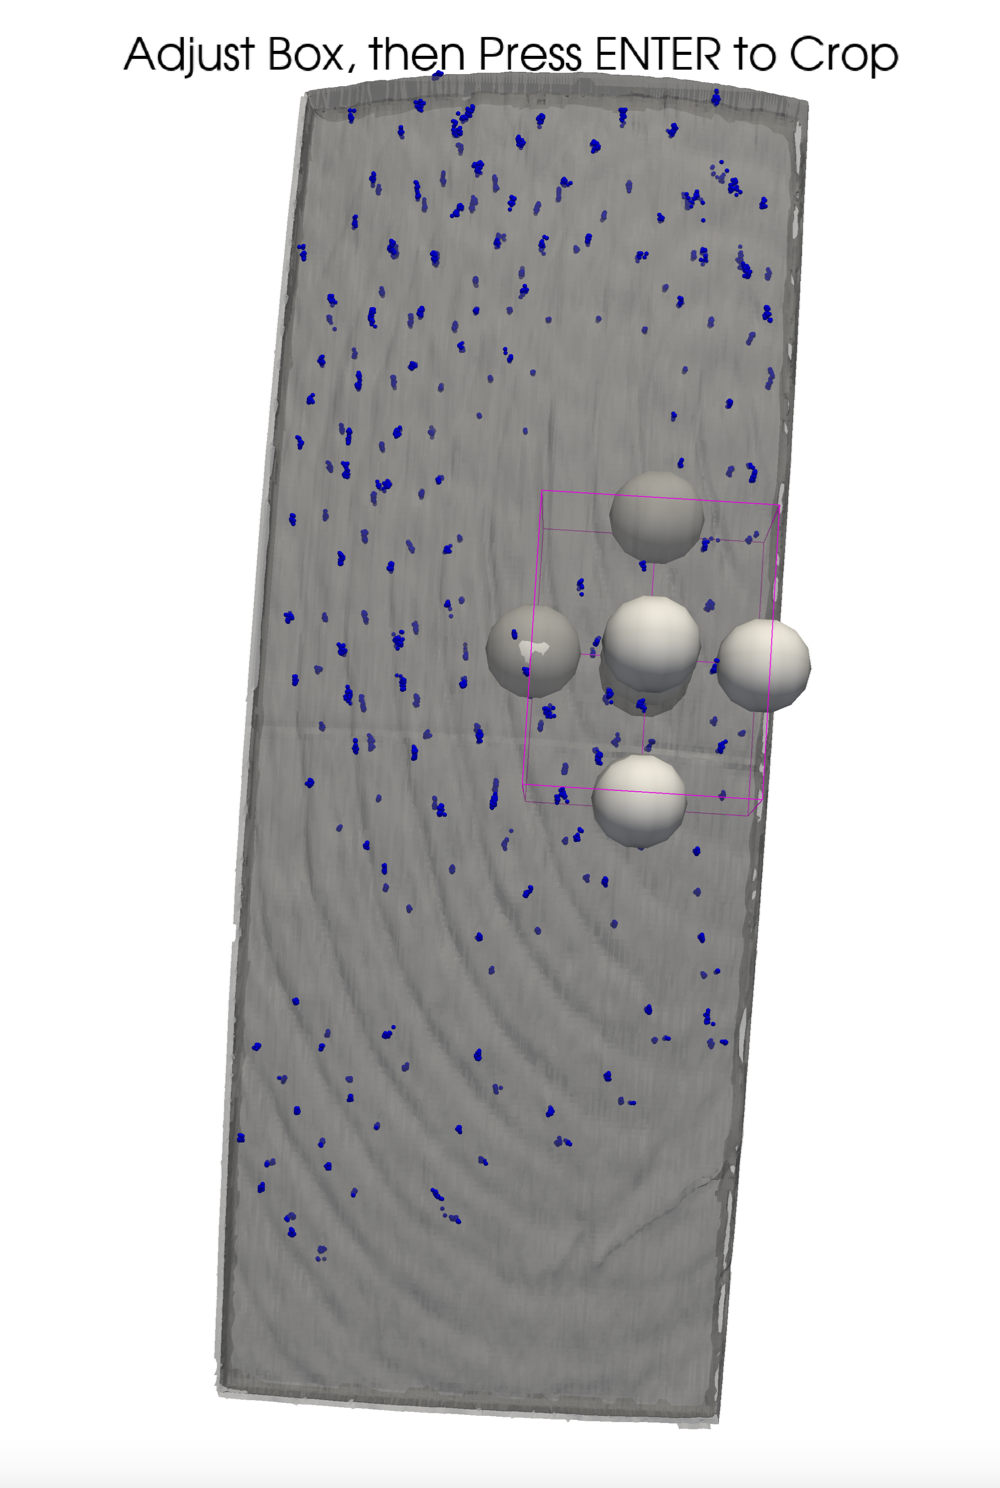
\includegraphics[width=\textwidth]{images/cropped_ROI.png}
        \caption{Cropped ROI for sweat duct subset.}
        \label{fig:additional_figure_1}
    \end{minipage}
    \hfill
    \begin{minipage}{0.41\textwidth}
        \centering
        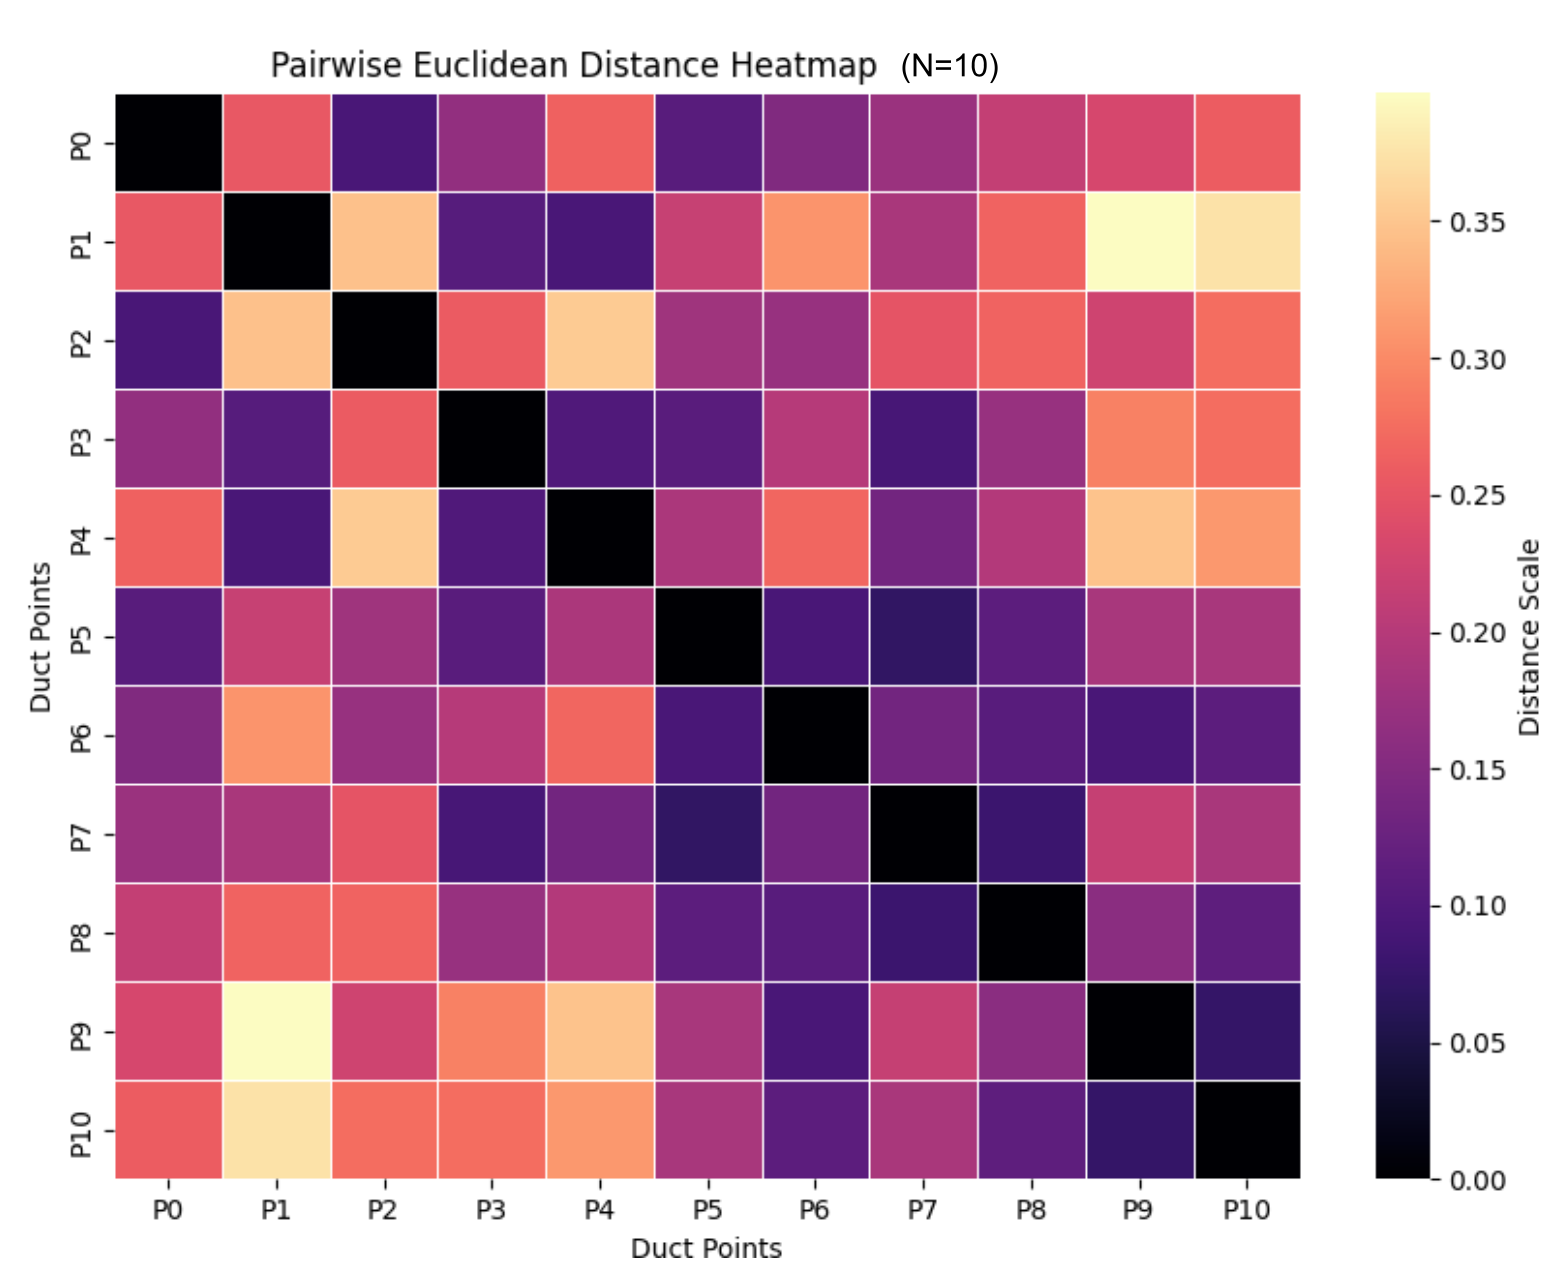
\includegraphics[width=\textwidth]{images/croppedSD-pairwise-heatmap.png}
        \caption{Pairwise heatmap for sweat duct subset.}
        \label{fig:additional_figure_2}
    \end{minipage}
    
    \vspace{0.5cm}
    
    \begin{minipage}{0.41\textwidth}
        \centering
        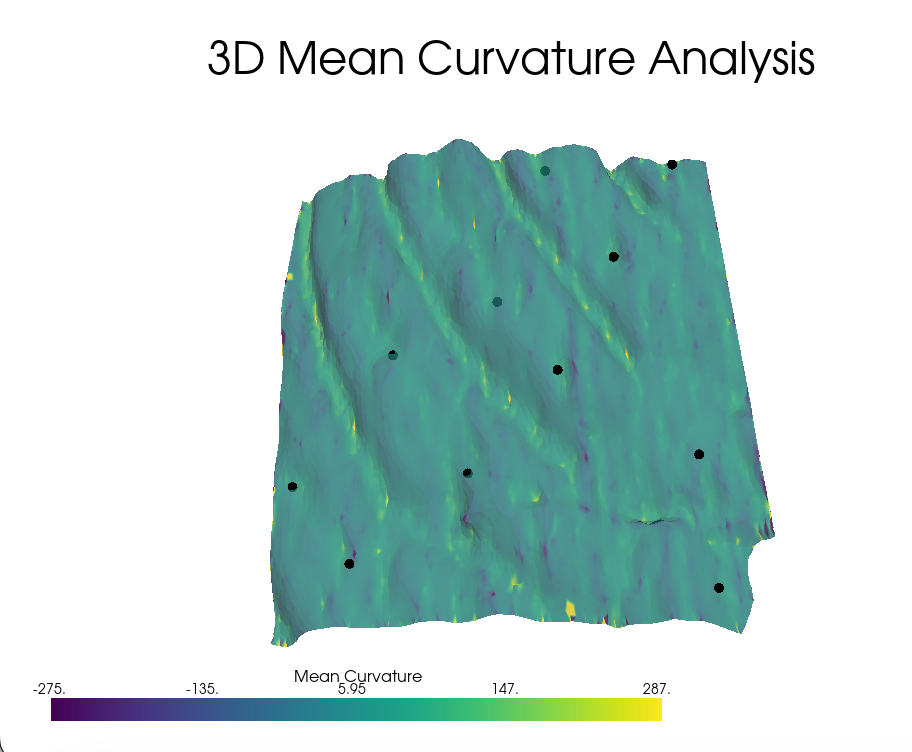
\includegraphics[width=\textwidth]{images/croppedSD_3D_mean_curvature.png}
        \caption{3D mean curvature for sweat duct subset.}
        \label{fig:additional_figure_3}
    \end{minipage}
    \hfill
    \begin{minipage}{0.41\textwidth}
        \centering
        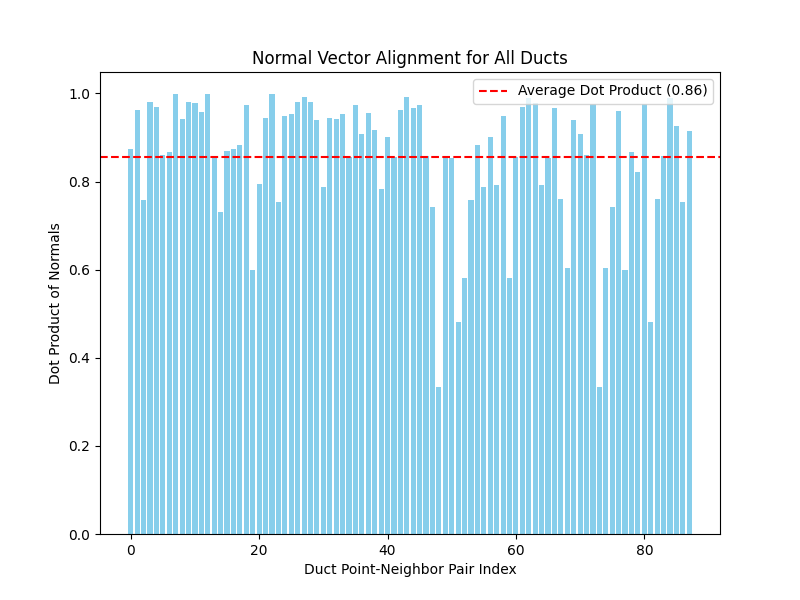
\includegraphics[width=\textwidth]{images/cropped_normal_dot_product.png}
        \caption{Normal vector dot product for sweat duct subset.}
        \label{fig:additional_figure_4}
    \end{minipage}
\end{figure}

\end{document}